\section{Kupfer-PVD}
\label{copperpvd}

Ein zweites PVD-System stellt Kupfer dar, wofür eine Vielzahl an unterschiedlichen Parametrisierungen vorliegen (Tabelle \ref{tab:copperpots}).
Es stellt sich die Aufgabe, eine passende Parametrisierung darunter zu suchen und zu entscheiden, inwiefern eine Vorauswahl anhand weniger Parameter \todo{chword} sinnvoll ist.
Kupfer bildet ebenfalls fcc-Kristalle, 

\begin{table}[hbtp]
  \caption[EAM-Parametrisierungen für Kupfersysteme]{EAM-Parametrisierungen für Kupfersysteme.}
  \label{tab:copperpots}
  \rowcolors{0}{white}{lightgray}
  \begin{tabularx}{\textwidth}{|lXc|}
    \hline
    \textbf{Bezeichnung} & \textbf{Anwendung \& Kommentare} & \textbf{Ref.} \\
    \hline
    CuAg.eam.alloy & Strukturelle und thermische Eigenschaften von \ce{Cu-Al} & \cite{williams_embedded-atom_2006} \\
    cu\_ag\_ymwu.eam.alloy & Mono-, Di-, Trimere und Inseln von \ce{Cu} auf \ce{Ag} & \cite{wu_cu/ag_2009} \\
    Cu\_smf7.eam & Oberflächen von \ce{Ni-Cu}-Legierungen bei \SI{800}{\kelvin} & \cite{foiles_calculation_1985} \\
    Cu\_u3.eam & Oberflächen und Bulks verschiedener Legierungen & \cite{foiles_embedded-atom-method_1986} \\
    Cu\_u6.eam & Aktivierungsenergie für Eigendiffusionen & \cite{adams_self-diffusion_1989} \\
    Cu-Zr\_2.eam.fs & Flüssige und amorphe \ce{Cu-Zr}-Legierungen & \cite{mendelev_development_2009} \\
    Cu-Zr.eam.fs & Flüssige und amorphe \ce{Cu-Zr}-Legierungen & \cite{mendelev_using_2007} \\
    Mendelev\_Cu2\_2012.eam.fs & Unterkühlte \ce{Al-Cu}-Schmelzen. Basiert auf \cite{mendelev_analysis_2008} & \cite{_interatomic_2014} \\
    \hline
  \end{tabularx}
  
\end{table}

\subsection{Voruntersuchungen}

Bei den Voruntersuchungen der strukturellen Eigenschaften konnten einige Parametersätze von LAMMPS nicht akzeptiert werden oder haben sich mit kryptischen Fehlern auf negative Speicherallokierungen aufgehangen.
Die Ergebnisse der drei verbliebenen Potentiale sind jedoch in guter Übereinstimmung mit Literaturwerten (Tabelle \ref{tab:copperpreresults}).
\todo{Dichte}Der Schmelzpunkt wurde jedoch nicht zuverlässig simuliert (Abbildung \ref{fig:copperthermo}).

\begin{table}[hbtp]
  %% \rowcolors{0}{white}{lightgray} 
  \caption[Eigenschaften von Gold]{Vergleich der Eigenschaften von Gold mit experimentellen und Literaturdaten als Voruntersuchung des PVD-Prozesses\todo[inline]{ref}}
  \label{tab:goldpreresults}
  \begin{tabularx}{\textwidth}{|lXXXX|}
    \hline
    \textbf{unters. Größe} & \textbf{Experiment} & \textbf{Cu\_smf7.eam} & \textbf{Cu\_u3.eam} & \textbf{Cu\_u6.eam} \\
    \hline
    Bindungslänge  &  \SI{2.556}{\angstrom} & \SI{2.558}{\angstrom} & \SI{2.558}{\angstrom} & \SI{2.558}{\angstrom} \\
    Koordination   &  \SI{12.00}{} & \SI{12.00}{} & \SI{12.00}{} & \SI{12.00}{} \\
    Dichte         & \SI{8.92}{\gram\per\cubic\centi\meter} & \SI{8.908}{\gram\per\cubic\centi\meter} & \SI{8.915}{\gram\per\cubic\centi\meter} & \SI{8.910}{\gram\per\cubic\centi\meter} \\
    \hline
  \end{tabularx}
\end{table}

\todo[inline]{Oberflächenvalidierung?}

\begin{figure}[tbp]
  \centering
  \captionsetup[subfigure]{singlelinecheck=false}
  \def\subfigwidth{7cm}
  \begin{subfigure}[t]{\subfigwidth}
    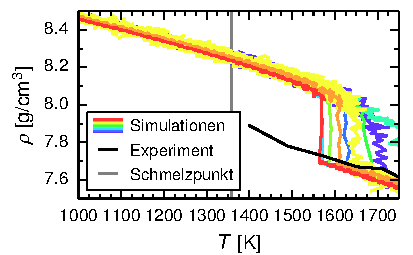
\includegraphics[width=\textwidth]{Cu_u6_meltingpoint}
    \subcaption{Phasenübergang mit Cu\_u6.eam bei unterschiedlichen $t_\text{relax}$}
  \end{subfigure}
  \hfill
  \begin{subfigure}[t]{\subfigwidth}
    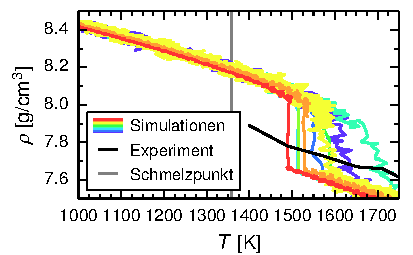
\includegraphics[width=\textwidth]{Cu_smf7_meltingpoint}
    \subcaption{Phasenübergang mit Cu\_smf7.eam bei unterschiedlichen $t_\text{relax}$}
  \end{subfigure}
  \caption[Abweichung der Schmelztemperaturen bei Kupfer-MD]{
    Abweichung der Schmelztemperatur mit verschiedenen Parametrisierungen.
    Experimentelle Werte von Brillo et al.\cite{brillo_density_2006}.
  }
  \label{fig:goldthermo}
\end{figure}

\subsection{Prozess-Simulation}

Äquivalent zur Vorgehensweise beim Gold-PVD-Prozess wurde ein Kupfer-PVD-Prozess gestartet
Zur Simulation eines Gold-PVD-Prozesses mit Parsivald wurden die untersuchten Potentialparameter sowie ein Kristallsubstrat eingelesen, ein Abscheidungsmodus mit zufälligen Auftreffpositionen in der xy-Ebene gewählt und Relaxationszeiten und Reaktionsnachbarschaftsgrößen gewählt, die in den vorheringen Tests als hinreichend ermittelt wurden.
Damit ergaben sich Reaktionsräume der Größe \SI{37x37x25}{\angstrom} mit jeweils ca. 1800 Atomen, Relaxationszeiten von \SI{1.4}{\nano\second} in \SI{1400}{} Simulationsschritten und Auftreffgeschwindigkeiten von \SI{4}{\angstrom/\pico\second}, die aus üblichen Sputterbedingungen stammen.\todo{wie berechnet?}
Die \SI{100x100}{\angstrom} breiten Kristalle werden perfekt fortgesetzt, wobei nach 10 Kristallschichten eine Rauheit von einem Atomdurchmesser vorliegt, was Übereinstimmung mit einem diffusionsdominierten Abscheidungsprozess zeigt.

\subsubsection{Strukturierte Substrate}

Als Stabilitätsprüfung wurden auch Abscheidungen auf strukturierten Substraten (Abbildung \ref{fig:coppersubstrate}) mit den gleichbleibenden Prozessbedingungen simuliert.
Es wurden Stufen und Spitzen mit Neigungen von jeweils \SI{15}{\degree}, \SI{20}{\degree}, \SI{30}{\degree}, \SI{45}{\degree}, \SI{60}{\degree} und \SI{90}{\degree} bei oben genannten Prozessbedingungen untersucht.
\todo{vorherige Relaxation?}

\begin{figure}[bt]
  \captionsetup[subfigure]{singlelinecheck=false}
  \def\subfigwidth{0.31\textwidth}
  \begin{subfigure}[t]{\subfigwidth}
    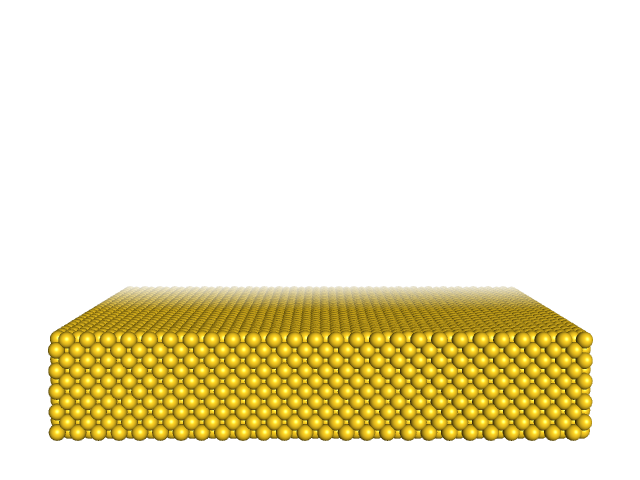
\includegraphics[width=\textwidth]{Au_substrate_flat}
    \subcaption{Glattes Gold-Substrat}
    \label{fig:coppersubstrate-a}
  \end{subfigure}
  \hfill
  \begin{subfigure}[t]{\subfigwidth}
    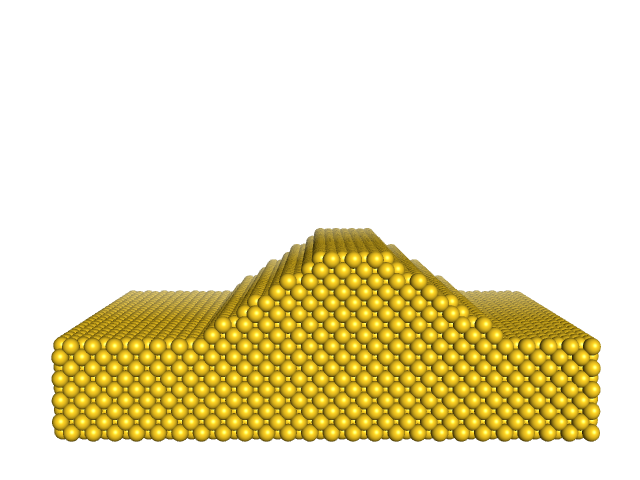
\includegraphics[width=\textwidth]{Au_substrate_step30}
    \subcaption{Gold-Stufe, \SI{30}{\degree}}
    \label{fig:coppersubstrate-b}
  \end{subfigure}
  \hfill
  \begin{subfigure}[t]{\subfigwidth}
    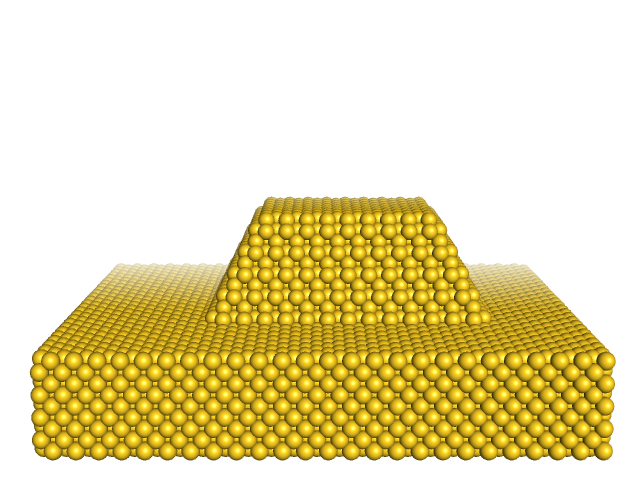
\includegraphics[width=\textwidth]{Au_substrate_tip60}
    \subcaption{Gold-Spitze, \SI{60}{\degree}}
    \label{fig:coppersubstrate-c}
  \end{subfigure}
  \caption[Strukturierte Coppersubstrate]{Coppersubstrate mit unterschiedlicher Struktur und Breite und Tiefe von \SI{100}{\angstrom}.
    Abscheidungen wurden auf glatten Substraten, Stufen und Spitzen vorgenommen.}
  \label{fig:coppersubstrate}
\end{figure}

\begin{figure}[bt]
  \captionsetup[subfigure]{singlelinecheck=false}
  \def\subfigwidth{0.31\textwidth}
  \begin{subfigure}[t]{\subfigwidth}
    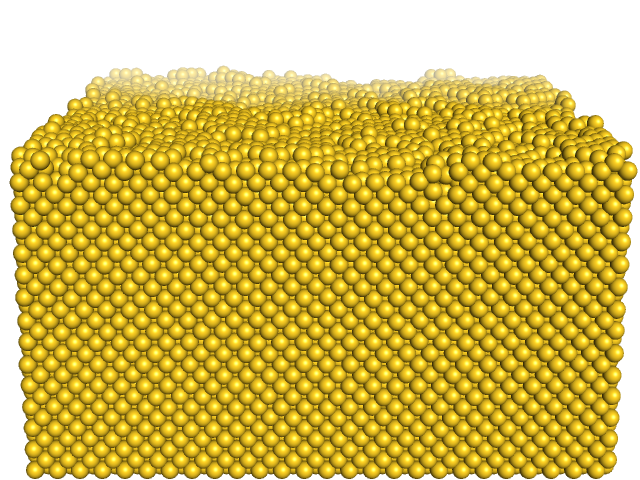
\includegraphics[width=\textwidth]{Au_deposition_flat}
    \subcaption{Abscheidung auf glattem Gold-Substrat}
    \label{fig:copperdepositions-a}
  \end{subfigure}
  \hfill
  \begin{subfigure}[t]{\subfigwidth}
    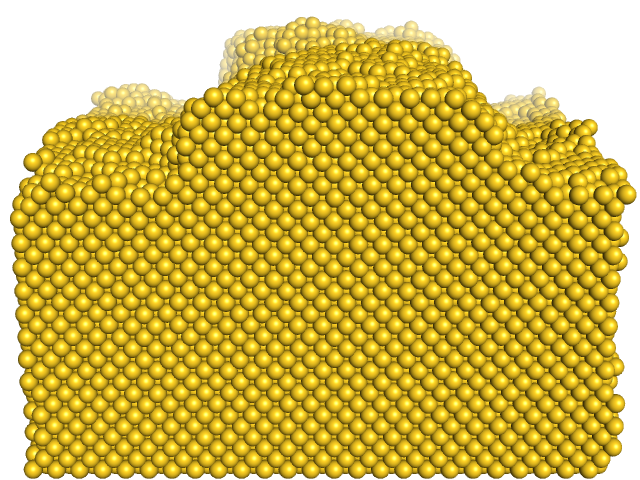
\includegraphics[width=\textwidth]{Au_deposition_step30}
    \subcaption{Abscheidung auf Gold-Stufe, \SI{30}{\degree}}
    \label{fig:copperdepositions-b}
  \end{subfigure}
  \hfill
  \begin{subfigure}[t]{\subfigwidth}
    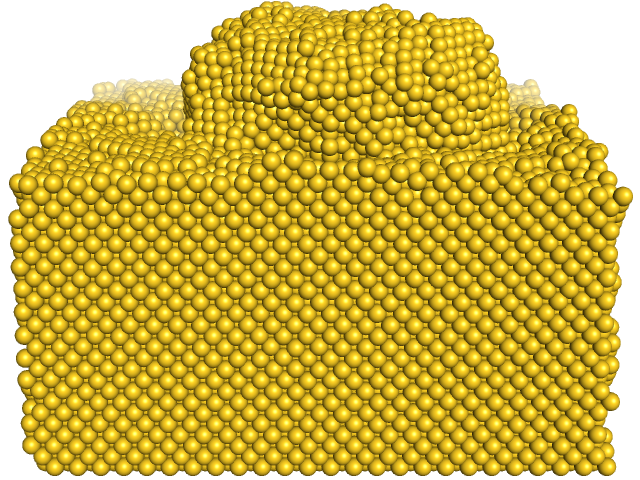
\includegraphics[width=\textwidth]{Au_deposition_tip60}
    \subcaption{Abscheidung auf Gold-Spitze, \SI{60}{\degree}}
    \label{fig:copperdepositions-c}
  \end{subfigure}
  \caption[Abscheidung auf strukturierten Substraten]{
    Ergebnis der Abscheidung.
    Die Substratstruktur bleibt erkennbar, wird aber nach oben verstärkt, ansonsten aber kristallin und glatt fortgesetzt.
  }
  \label{fig:copperdepositions}
\end{figure}

Das Kristallsubstrat wird auch hier fortgesetzt, jedoch verstärken sich Neigungswinkel an Stufen und Spitzen zunehmend.
Nach längeren Laufzeiten entstehen somit Überhänge, die durch Abschluss von unten zu Hohlräumen innerhalb der Struktur führen, welche in der Realität durch thermische Relaxation geschlossen würden.
Dahinter steht einerseits die Notwendigkeit, Gold-Atome bei Ankunft auf der Oberfläche ausreichend diffundieren zu lassen, was beim aktuellen Modell nur innerhalb der Reaktionsraumgrenzen geschieht.

Andererseits liegt ein methodischer Fehler bei Nutzung von Binning-Methoden vor:
Die Oberfläche wird aus algorithmischen Gründen nur entlang der z-Achse bestimmt, woraufhin das neue Atom oberhalb eines Referenzatomes auf der Oberfläche platziert wird.
An Stufen und Kanten werden hierbei höhere Reaktionsorte bevorzugt, an denen das Atom mit \todo{phrasing}statistischer Wahrscheinlichkeit verbleibt.

Einen Lösungsansatz stellt die ausführliche Parametrisierung der Oberfläche dar, beispielsweise per Alpha-Form (siehe Abschnitt \ref{dataalphaform}, über die man die Ereigniswahrscheinlichkeit entsprechend der Einbettungsenergie variierte, angenähert über die Oberflächenkrümmung.


%% \begin{table}[H]
%%   %% \oddrowcolors
%%   \begin{tabularx}{0.8\textwidth}{|XXX|}
%%     \hline
%%     sdf & fds & sdf \\
%%     \hline
%%     sdf & fds & sdf \\
%%     sdf & fds & sdf \\
%%     sdf & fds & sdf \\
%%     \hline
%%   \end{tabularx}
%% \end{table}

%% \begin{table}[H]
%%   \oddrowcolors
%%   \begin{tabularx}{0.8\textwidth}{|XXX|}
%%     \hline
%%     sdf & fds & sdf \\
%%     \hline
%%     sdf & fds & sdf \\
%%     sdf & fds & sdf \\
%%     sdf & fds & sdf \\
%%     \hline
%%   \end{tabularx}
%% \end{table}

%% \begin{table}[H]
%%   \evenrowcolors
%%   \begin{tabularx}{0.8\textwidth}{|XXX|}
%%     \hline
%%     sdf & fds & sdf \\
%%     \hline
%%     sdf & fds & sdf \\
%%     sdf & fds & sdf \\
%%     sdf & fds & sdf \\
%%     \hline
%%   \end{tabularx}
%% \end{table}

%% \setlength{\arrayrulewidth}{0.6pt}
%% \begin{table}[H]
%%   \oddrowcolors
%%   \begin{tabularx}{0.8\textwidth}{|XXX|}
%%     \hline
%%     sdf & fds & sdf \\
%%     \hline
%%     sdf & fds & sdf \\
%%     sdf & fds & sdf \\
%%     sdf & fds & sdf \\
%%     \hline
%%   \end{tabularx}
%% \end{table}

%% \begin{table}[!ht]
%%   \centering

%%   \caption{Abschätzung der Komplexität für verschiedene Datenstrukturen und Operationen}
%%   \label{tab:dataruntimes}
%%   \begin{tabularx}{\textwidth}{|X|*8c|}
%%     \hline
%%     \textbf{Datenstr.} & Konstr.         & Einfüg.         & Modif.          & Entf.           & Ortss.                     & NB-Su.              & Oberfl.        & RAM                         \\
%%     \hline
%%     Atomlisten         & \cG{$n$}        & \cG{$1$}        & \cG{$1$}        & \cG{$1$}        & \cR{$n$}                   & \cR{$n$}            & \cR{$n$}       & \cG{$n$}                    \\
%%     NB-Listen          & \cY{$n\log{n}$} & \cR{$n$}        & \cR{$n$}        & \cR{$n$}        & \cR{$n$}                   & \cG{$1$}            & \cR{$n$}       & \cR{$\frac{r_c^3}{s^3}n^2$} \\
%%     Binning            & \cG{$n$}        & \cG{$1$}        & \cG{$1$}        & \cG{$1$}        & \cG{$r_s^3$}               & \cG{$r_s^3$}        & \cR{$c$}       & \cY{$n+c$}                  \\
%%     Octree             & \cY{$n\log{c}$} & \cY{$\log{c}$}  & \cY{$\log{c}$}  & \cG{$1$}        & \cY{$r_s^3\log{c}$}        & \cY{$r_s^3\log{c}$} & \cY{$\log{c}$} & \cY{$n+c^\frac{2}{3}$}      \\
%%     k-d-Baum           & \cY{$n\log{n}$} & \cY{$\log{n}$}  & \cY{$\log{n}$}  & \cY{$\log{n}$}  & \cY{$r_s^3\log{n}$}        & \cY{$r_s^3\log{n}$} & \cY{$\log{n}$} & \cG{$n$}                    \\
%%     Delaunay           & \cY{$n\log{n}$} & \cY{$k\log{k}$} & \cY{$k\log{k}$} & \cY{$k\log{k}$} & \cG{$r_s^3+n^\frac{1}{3}$} & \cG{$r_s^3$}        & \cG{$1$}       & \cY{$nk$}                   \\
%%     \hline
%%     %Atomfeld          & \cG{$n$}        & \cG{$1$}        & \cG{$1$}        & \cG{$1$}        & \cR{$n$}                   & \cR{$n$}            & \cR{$n$}       & \cG{$n$}                    \\
%%   \end{tabularx}
%%   \vspace{1em}
%%   \hspace{0.15\textwidth}
%%   \begin{tabularx}{0.6\textwidth}{|C|C|C|}
%%     \hline
%%     \cG{optimal} & \cY{vertretbar} & \cR{ineffizient} \\
%%     \hline
%%   \end{tabularx}

%%   \vspace{1em}

%%   \oddrowcolors
%%   \caption{Symbole für Laufzeit- und Speicherabschätzungen}
%%   \label{tab:datasymbols}
%%   \begin{tabularx}{\textwidth}{|cX|cX|}
%%     \hline
%%     \textbf{Symbol} & \textbf{Bedeutung}                 & \textbf{Symbol} & \textbf{Bedeutung} \\
%%     \hline
%%     \BigO{}         & Worst-Case-Komplexität             & $n$             & Zahl der Atome     \\
%%     $k$             & Zahl von Nächstnachbarn            & $b$             & Zahl der Bins      \\
%%     $k_r$           & Zahl von Nachbarn mit $d \leq r_c$ & $r_c$           & Cutoff-Radius      \\
%%     $r_s$           & Suchradius                         & $s$             & lineare Raumgröße  \\
%%     \hline
%%   \end{tabularx}

%% \end{table}
